\documentclass[10pt,a4paper]{article}
\usepackage[utf8]{inputenc}
\usepackage{amsmath}
\usepackage{amsfonts}
\usepackage{amssymb}
\usepackage{graphicx}
\usepackage{framed}
\usepackage{float}
\author{Paul Cowie \and Jacob Ford \and Nicole Munro \and William Kavanagh \and Ben Procter \and Pregashni Mohanarajah }
\date{}
\title{Team Six: IS(H) AX1, Report 1}
\begin{document}
\maketitle

\section*{Introduction}
The design process originated with the idea that to set our project aside from the others, we needed two key aspects:
Firstly, we needed to provide a unique method of searching which makes our service stand out from its numerous competitors and secondly, we needed a distinctive visual design to make the system desirable to use.

\section*{Functional Design}
Our product does not just search along a single dimension. Where other services allow users to only search and order results by only one category, such as price or average user rating, we allow users to rate how important a series of ‘keyword’ criteria are to them, as well as offering the functionality of more conventional services.

Our service works by allowing users the ability to search available options for what is important to them such as price, location, cuisine type or even restaurant name. Through a drag and drop ‘pinboard’ interface, users will be able to prioritise their keywords allowing them to search and customise results to meet their personal needs.

The pinboard functionality also gives users the ability to rank the importance of customisations, for example, if a user is less concerned with restaurant proximity, then they are able to convey this allowing the system to reprioritise customisations to make the results more indicative of user desires.

\section*{Visual Design}
In order to create our distinctive algorithmic approach, we produced and analysed a series of alternative ideas, comparing their respective pros and cons. Some such alternatives included spider diagrams and a ‘word cloud’ approach. This approach seemed favourable, however we eventually decided upon the multi dimensional search interface. When left with only two design options, we compared at length the which aspects of both designs were most effective merging these into what would become our final design. By performing A/B analysis, we ensured that the best features of all versions were successfully incorporated.

We knew that to be effective our service needed to stand out visually, but to decide on the visual aspects of the design before we had agreed upon the overall approach would be foolish. We knew that the unique aspect of our design was the ability for multi-dimensional searching and so the first elements of our user-interface had to incorporate the searching for keywords (or ‘tags’) and a large drag and drop interface to allow for the ranking of these tags. Rather than overcomplicating the process for the users we decided to leave these elements very simple and stripped back. This meant that the space for search results was open for visual flair. We came up with several different ideas for displaying the results and incorporated the positive aspects into a single design. By sketching out wireframes we were able to compare the different designs effectively. The speed with which we could create new designs allowed for a very smooth iterative process which ensured we efficiently came to decisions as a group in spite of contrasting opinions.

Our final design has colourful hexagons cascading smoothly across the screen, displaying our results in order based on adherence to the keywords. The intention was to clearly display the results in a distinctive way that also showed how firmly they correspond with the user’s search query. By having the hexagons all coloured with an intensity that denoted a restaurant's correlation to the user’s query we found a way that makes the design visually appealing and highly functional. We believe that the way our results are displayed, in an aesthetically pleasing, tessellating  design is unique and provides our product with a distinctive and strong brand image.

\begin{figure}[H]
	\begin{center}
		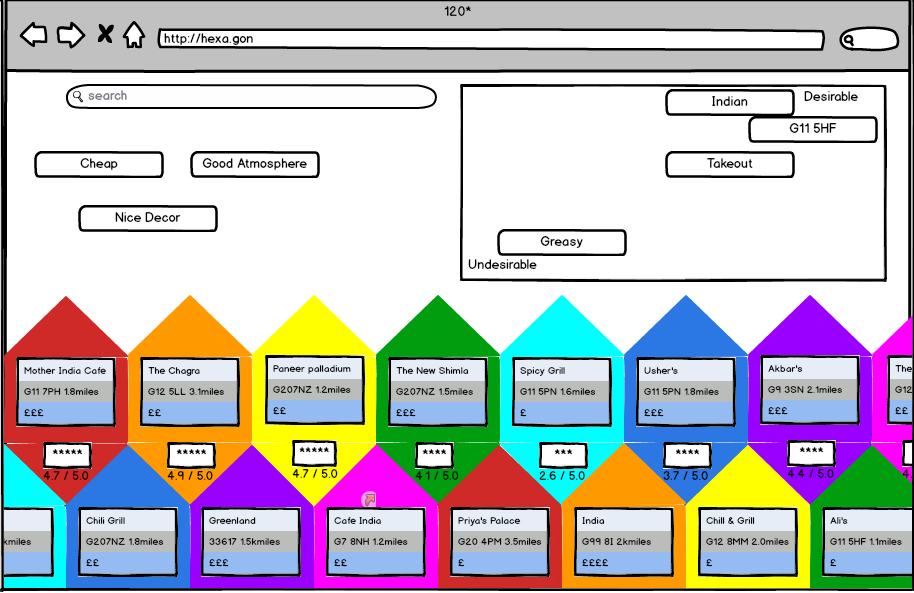
\includegraphics[scale=0.37]{Screenshot.png}
		\caption{Mockup of main page}
		\label{figure:calc-1}
	\end{center}
\end{figure}

\section*{User Stories}
Our design is highly functional and caters to a large portion of the available market, but we identified a few target user groups that would benefit most from our design. Our target users fall under three categories: People visiting Glasgow who are not familiar with the city, people who like to plan ahead, and people with very specific tastes. People visiting the city would not be likely to know where to find places to eat and would therefore find our product useful. People planning ahead will be able to find a place to eat that will be close to where they know they will be later. People with specific tastes will be able to make good use of the pinboard function to ensure that they can avoid restaurants that serve food they don’t like.

To carry the design process forward, we needed to display how we were catering to our audience, so we created some user personas and scenarios. The following are the user personas which we created to display what customers we envisage as using our system.

\begin{framed}
Trevor Hogan is an American in Glasgow on a business trip. He likes chippies, since he can rarely find them back home. He also strongly dislikes spicy food, so he wants to avoid that as much as possible. He is 26 years old.

Mandy Uri is a 22 year old student who was born in Glasgow. She likes tennis and working hard. She likes Italian food, and often wants to plan to go to Italian restaurants after finishing a tennis match.

Maceij Vytotsky is a Russian immigrant who only likes to eat Eastern-European food when he goes out to eat, which can be difficult to find in Glasgow. He likes DOTA, and listening to old folk songs. He is 54 years old, and works as a fisherman, so he often isn't able to plan to eat while working.
\end{framed}


\section*{User Scenarios}
We generated some example scenarios which portray the situations in which our users will interact with our product.

\begin{framed}
Trevor just got out of his business meeting and is hungry. He opens the app, drags 'chippie' to desirable and 'spicy' to undesirable. The website automatically takes his location and returns hexagons representing chippies near him, but not ones that are known for their spicy food. He clicks on a high-rated one and opens the map from his current location to the restaurant.

Mandy Uri knows she will be hungry after her tennis match on courts near the Kelvingrove park. She opens the website in the morning, entering her preferences (italian) as well as the location of her tennis match. She won't want to go to a nice restaurant all sweaty after a hard tennis match, so she enters 'cheap' as well. The website gives her multiple options for cheap italian restaurants and takeouts near the tennis courts.

Maceij Vytotsky is tired from a long day of fishing and can't be bothered cooking himself dinner. He opens the app, and being an old russian national, drags several types of foreign cuisine to the undesirable section of the pinboard. He is in the mood for something nice, so he enters the keyword 'fancy' as well as 'russian' and 'eastern european' in the upper right corner of the pinboard. Hexagons for Russian Restaurants near him appear and he chooses a nice cafe.
\end{framed}

\section*{Requirements}
\subsection*{Functional}
Once we had formed our user personas and their accompanying scenarios we were able to formally write up the functional and non-functional requirements for our system. The following are the functional requirements we have identified for our design:

\begin{itemize}
	\item Add tags to a scale to determine restaurant rankings.
	\item Access JustEat page/website when selected.
	\item Use a map to find directions to a chosen restaurant.
	\item View metrics such as average price/average ranking at a glance.
	\item Background colour of each result is shaded in such a way as to display the relevance of the result to the user, based on the tags they chose and their location.
	\item Default location to the user's current location, but allow this to be changed if they want to plan from somewhere else.
\end{itemize}
	
\subsection*{Non-Functional}
We also outlined the non-functional requirements of our design:

\begin{itemize}
	\item Access on desktop/mobile/tablet.
	\item Small page weight, to reduce data usage and download time when using a mobile network.
\end{itemize}

\section*{Conclusion}
In conclusion, our project offers an interesting new approach to search, backed by a distinctive visual design. Ease of use combined with unique functionality ensures that our website will be useful and attractive to each of our target user groups.


\end{document}